%%%%%%%%%%%%%%%%%%%%%%%%%%%%%%%%%%%%%%%%%
% Beamer Presentation
% LaTeX Template
% Version 1.0 (10/11/12)
%
% This template has been downloaded from:
% http://www.LaTeXTemplates.com
%
% License:
% CC BY-NC-SA 3.0 (http://creativecommons.org/licenses/by-nc-sa/3.0/)
%
%%%%%%%%%%%%%%%%%%%%%%%%%%%%%%%%%%%%%%%%%

%----------------------------------------------------------------------------------------
%	PACKAGES AND THEMES
%----------------------------------------------------------------------------------------

\documentclass[notes]{beamer}  

\mode<presentation> {

% The Beamer class comes with a number of default slide themes
% which change the colors and layouts of slides. Below this is a list
% of all the themes, uncomment each in turn to see what they look like.

%\usetheme{default}
%\usetheme{AnnArbor}
%\usetheme{Antibes}
%\usetheme{Bergen}
%\usetheme{Berkeley}
%\usetheme{Berlin}
%\usetheme{Boadilla}
%\usetheme{CambridgeUS}
%\usetheme{Copenhagen}
%\usetheme{Darmstadt}
%\usetheme{Dresden}
%\usetheme{Frankfurt}
%\usetheme{Goettingen}
%\usetheme{Hannover}
%\usetheme{Ilmenau}
%\usetheme{JuanLesPins}
%\usetheme{Luebeck}
\usetheme{Madrid}
%\usetheme{Malmoe}
%\usetheme{Marburg}
%\usetheme{Montpellier}
%\usetheme{PaloAlto}
%\usetheme{Pittsburgh}
%\usetheme{Rochester}
%\usetheme{Singapore}
%\usetheme{Szeged}
%\usetheme{Warsaw}

% As well as themes, the Beamer class has a number of color themes
% for any slide theme. Uncomment each of these in turn to see how it
% changes the colors of your current slide theme.

%\usecolortheme{albatross}
%\usecolortheme{beaver}
%\usecolortheme{beetle}
%\usecolortheme{crane}
%\usecolortheme{dolphin}
%\usecolortheme{dove}
%\usecolortheme{fly}
%\usecolortheme{lily}
%\usecolortheme{orchid}
%\usecolortheme{rose}
%\usecolortheme{seagull}
%\usecolortheme{seahorse}
%\usecolortheme{whale}
%\usecolortheme{wolverine}

%\setbeamertemplate{footline} % To remove the footer line in all slides uncomment this line
%\setbeamertemplate{footline}[page number] % To replace the footer line in all slides with a simple slide count uncomment this line

%\setbeamertemplate{navigation symbols}{} % To remove the navigation symbols from the bottom of all slides uncomment this line
}

\usepackage{graphicx} % Allows including images
\usepackage{booktabs} % Allows the use of \toprule, \midrule and \bottomrule in tables
\usepackage[slovene]{babel}
\usepackage[T1]{fontenc}
\usepackage{textcomp}
\usepackage{tabularx}
\usepackage{pgfpages}
\usepackage{verbatim}
\usepackage{listings}

\setbeamertemplate{caption}{\raggedright\insertcaption\par}
%\setbeameroption{hide notes}
\setbeameroption{show notes on second screen}
\setbeamertemplate{note page}{\pagecolor{yellow!5}\vfill\insertnote\vfill}
%----------------------------------------------------------------------------------------
%	TITLE PAGE
%----------------------------------------------------------------------------------------

\title[CI/CD poslovno kritičnih aplikacij]{Neprekinjena integracija in dostava poslovno kritičnih aplikacij
} % The short title appears at the bottom of every slide, the full title is only on the title page

\author{Jakob Maležič} % Your name
\institute[] % Your institution as it will appear on the bottom of every slide, may be shorthand to save space
{
Fakulteta za računalništvo in informatiko \\ % Your institution for the title page
\medskip \\ % Your email address
\textit{jm6421@student.uni-lj.si} \\ % Your email address
}
\date{\today} % Date, can be changed to a custom date

\begin{document}

\begin{frame}
\titlepage % Print the title page as the first slide

% \note[item]{}
\note[item]{Pozdravljeni, moje ime je Jakob Maležič in danes Vam bom predstavil svoje magistrsko delo z naslovom Neprekinjena integracija in dostava poslovno kritičnih aplikacij.}

\end{frame}

% \begin{frame}
% \frametitle{Kazalo} % Table of contents slide, comment this block out to remove it
% \tableofcontents % Throughout your presentation, if you choose to use \section{} and \subsection{} commands, these will automatically be printed on this slide as an overview of your presentation
% \end{frame}

%----------------------------------------------------------------------------------------
%	PRESENTATION SLIDES
%----------------------------------------------------------------------------------------

\begin{frame}
\frametitle{Uvod}
\begin{columns}

\column{.6\textwidth} % Left column and width
\begin{itemize}
    \item \textbf{neprekinjena integracija} (ang. \textit{Continuous Integration - CI}) - redno dodajanje in združevanje sprememb programske kode
    \item \textbf{neprekinjena dostava} (ang. \texit{Continuous Delivery - CD}) - dostava programske kode naročniku
    \item \textbf{poslovno kritične aplikacije} - ključne za delovanje poslovnega procesa podjetja
\end{itemize}

\column{.4\textwidth}
\begin{figure}[htbp]
\begin{center}
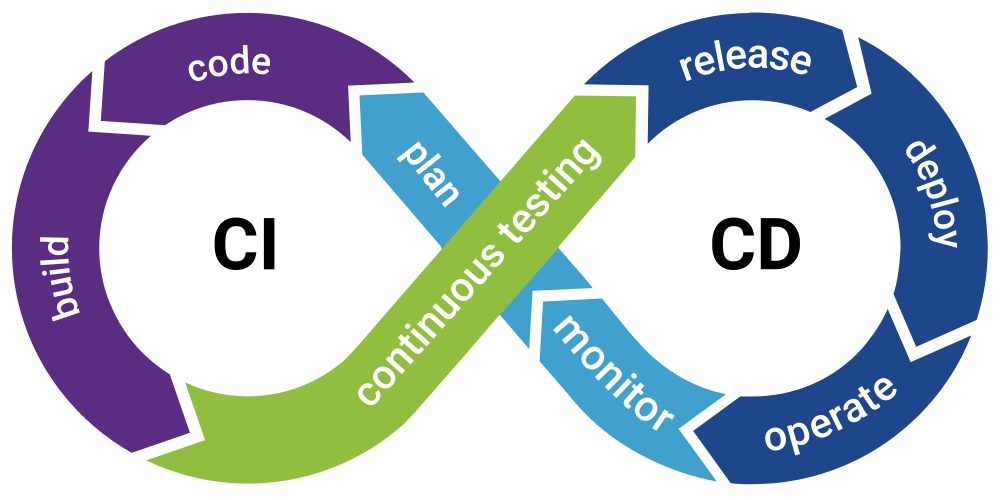
\includegraphics[scale=0.12]{figs/cicd.png}
% \caption{DevOps.}
% https://www.synopsys.com/glossary/what-is-cicd.html
\label{slika1}


\end{center}
\end{figure}


\end{columns}

\note[item]{Zaradi visoke konkurence na trgu programske opreme organizacije namenjajo veliko pozornosti pospešitvi razvoja in dostave kakovostnih aplikacij.}
\note[item]{Neprekinjena integracija je v tej industriji razširjena razvojna praksa, ki vzpodbuja redno dodajanje in združevanje sprememb programske kode. To omogoča podjetjem, da skrajšajo čas in povečajo pogostost razvojnega cikla, izboljšajo kakovost aplikacij in povečajo produktivnost razvojne ekipe.}
\note[item]{Neprekinjena dostava pa je metodologija, ki si prizadeva zagotoviti, da je aplikacija vedno pripravljena za namestitev in dostavo naročniku oziroma uporabnikom.}
\note[item]{Poseben primer aplikacij pa predstavljajo poslovno kritične aplikacije, ki so ključne za delovanje poslovnega procesa podjetja.
% Odpoved ali prekinitev delovanja takšnih aplikacij lahko potencialno povzroči veliko finančno škodo ali škoduje ugledu podjetja.
Zato je potrebno proces CI/CD pri takšnih aplikacijah ustrezno prilagoditi, da zadostuje vsem varnostnim zahtevam.}

\end{frame}

%------------------------------------------------

\begin{frame}
\frametitle{DevOps}


\begin{columns}

\column{.6\textwidth} % Left column and width
\begin{itemize}
    \item zbirka praks razvoja programske opreme
    \item vzpodbuja delitev odgovornosti med vse ekipe
    \item meje med različnimi vlogami članov razvojne ekipe se zabrisujejo
    \item dostava operativnih funkcij za delo s kodo naročniku
\end{itemize}

\column{.4\textwidth}
\begin{figure}[htbp]
\begin{center}


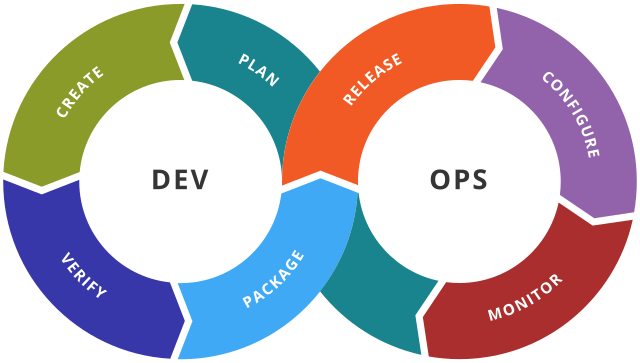
\includegraphics[scale=0.18]{figs/devops.png}
% \caption{DevOps.}
% https://en.wikipedia.org/wiki/DevOps_toolchain#/media/File:Devops-toolchain.svg
\label{slika1}


\end{center}
\end{figure}


\end{columns}

\note[item]{Omenjene prakse pa združuje zbirka razvojnih praks imenovana DevOps, ki vzpodbuja delitev odgovornosti med vse ekipe celotnega življenjskega cikla razvoja programske opreme.}
\note[item]{To pomeni, da se meje med različnimi vlogami postopno zabrisujejo, saj člani operativne ekipe prevzemajo naloge, ki so tradicionalno bolj usmerjene v razvijalce, in člani razvojne ekipe prevzemajo naloge, ki so tradicionalno bolj namenjene članom operativne ekipe.}
\note[item]{Zato je poleg programske opreme, naročniku ključno dostaviti tudi operativne funkcije za delo s kodo, enostavno namestitev aplikacij v več različnih okolji, možnost prenosa kode k drugemu izvajalcu in podobno.}
\end{frame}

%------------------------------------------------

\begin{frame}
\frametitle{Neprekinjena integracija}

\begin{columns}

\column{.3\textwidth} % Left column and width
\begin{itemize}
    \item centralni repozitorij
    \item orodje za gradnjo
    \item orodje za preizkušanje
\end{itemize}

\column{.7\textwidth} % Right column and width
\begin{figure}[htbp]
\begin{center}
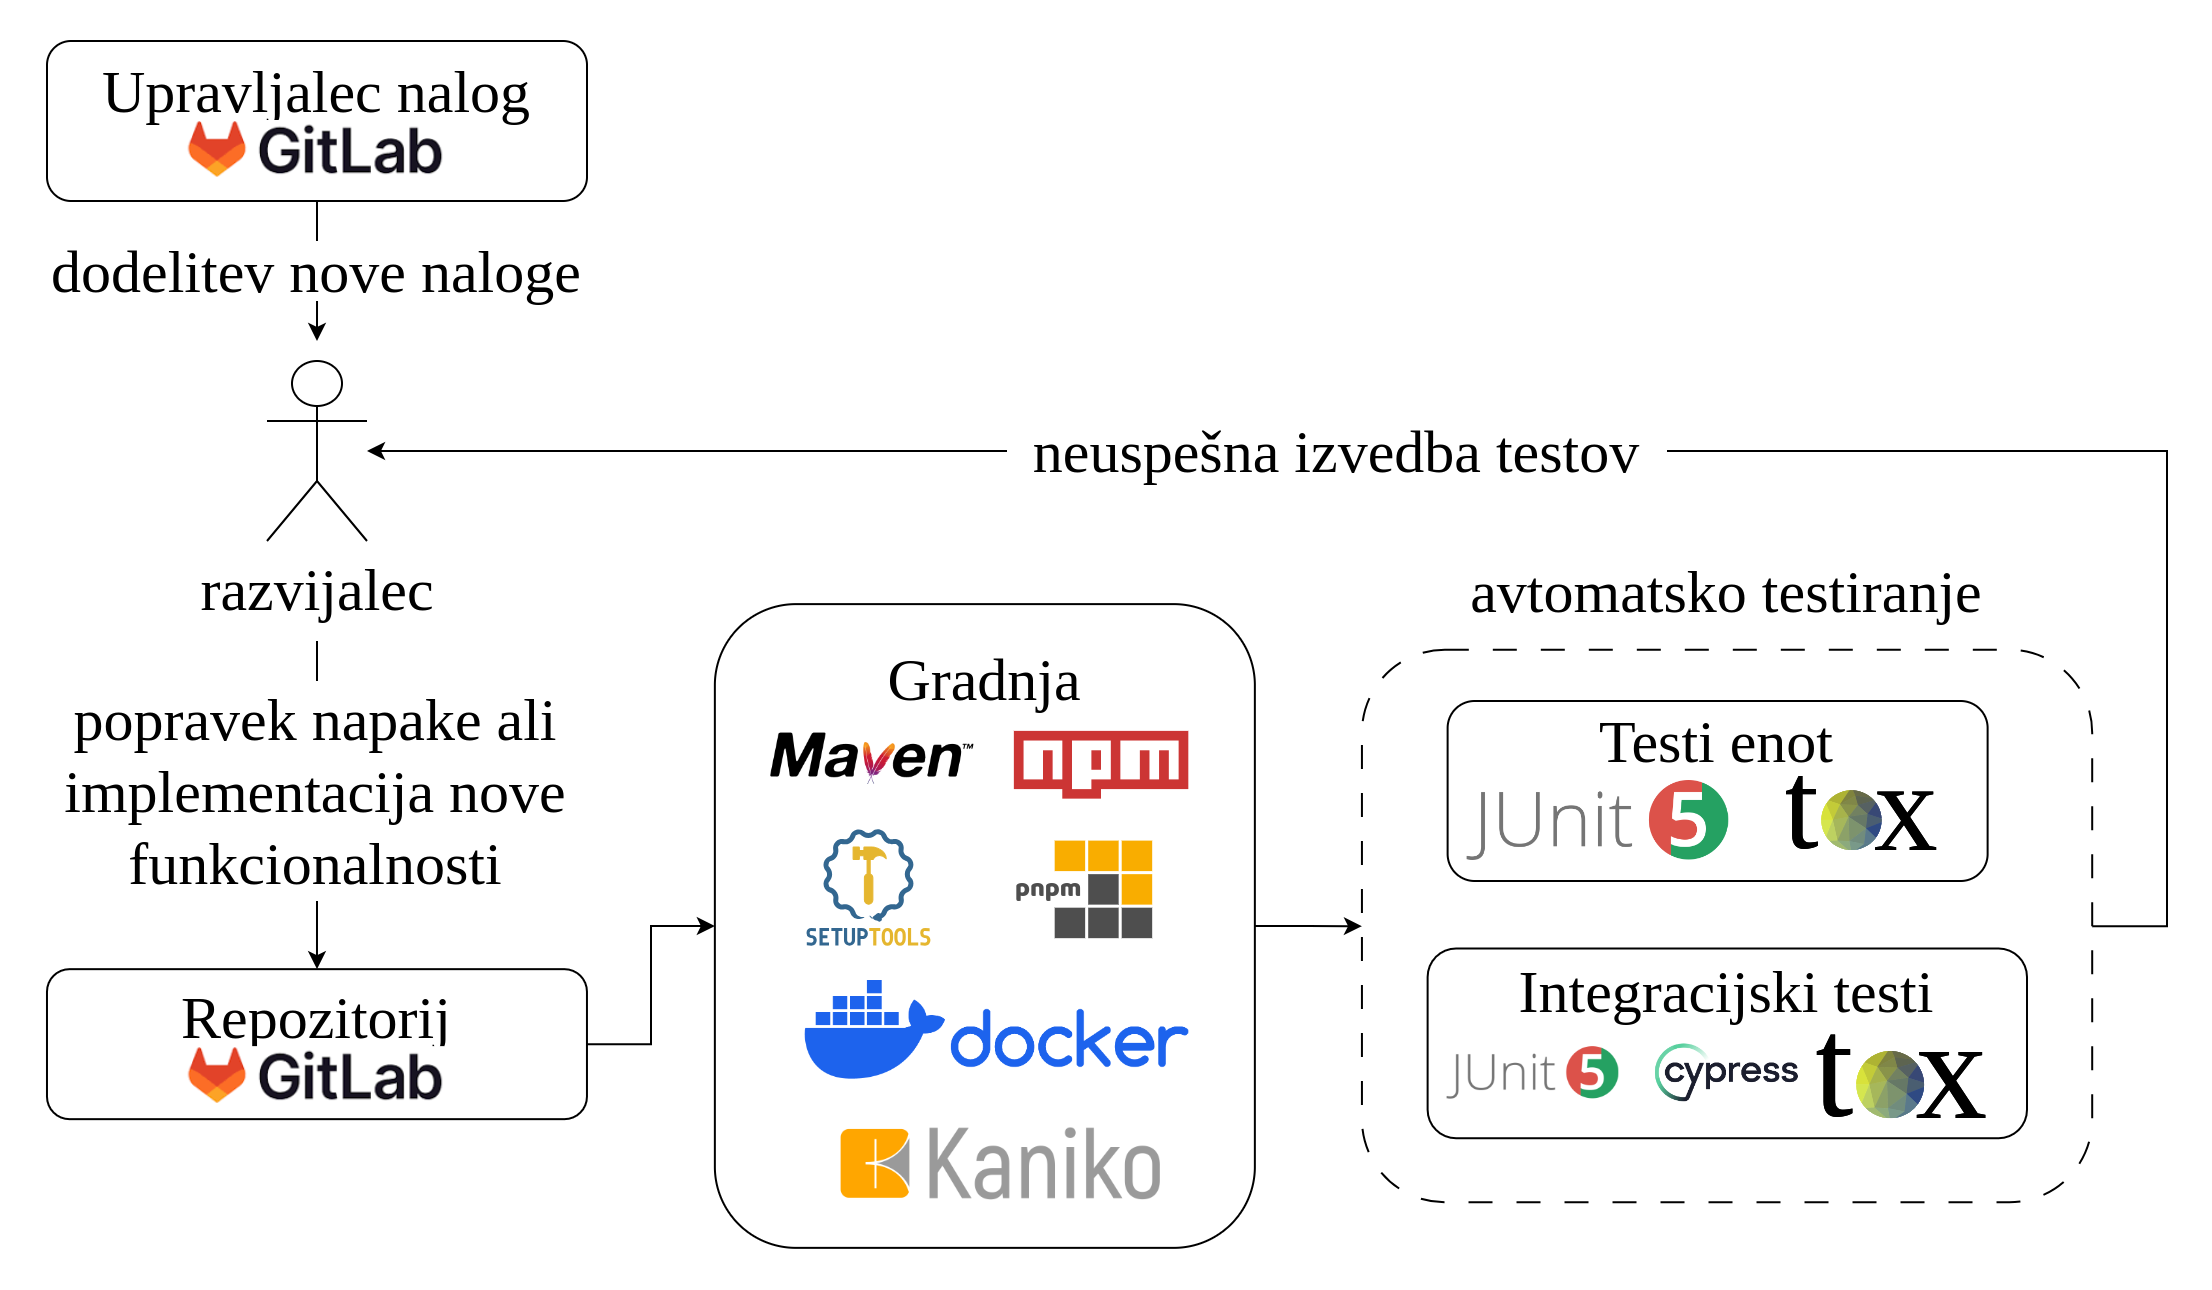
\includegraphics[scale=0.1]{figs/diagram-neprekinjene-integracije-2.png}
% \caption{Pregled podatkov iz strani Kaggle.}
\label{slika1}

\end{center}
\end{figure}

\end{columns}

\note[item]{Sistem neprekinjene integracije sestavljajo trije glavni elementi:}
\note[item]{centralni repozitorij, kamor razvijalci oddajajo svoje spremembe kode}
\note[item]{orodje za avtomatizacijo gradnje, ki je odgovorno za avtomatsko gradnjo in objavljanje posodobljene kode}
\note[item]{orodja za preizkušanje, ki izvajajo avtomatsko testiranje na posodobljeni kodi in s tem zagotavljajo, da ta deluje pravilno in dosega zahtevane standarde kakovosti}


\end{frame}

%------------------------------------------------

\begin{frame}
\frametitle{Neprekinjena dostava}

\begin{itemize}
    \item zmanjšanje časa med pisanjem kode in njene dostave končnim uporabnikom
    \item neprekinjena integracija
    \item izdajanje novih različic
    \item dostava izvorne kode naročniku
    % \item zagotavljanje ponovljive gradnje aplikacije (ang. \textit{reproducible build})
\end{itemize}


\note[item]{Cilj neprekinjene dostave je zmanjšanje časa med pisanjem kode in njene dostave končnim uporabnikom, obenem pa zagotavljanje visoke kakovosti in zanesljivosti.}
\note[item]{Neprekinjena dostava ima zato širši pomen, saj vključuje neprekinjeno integracijo, izdajanje novih različic in dostavo izvorne kode naročniku.}
\note[item]{Dostava izvorne kode je koristna tako za naročnika kot tudi za podjetje, ki je napisalo izvorno kodo.}
\note[item]{Za naročnika je koristna, ker ni več odvisen od podjetja z vidika posodobitev in lahko najame drugo podjetje ali pa ta del prevzame sam.}
\note[item]{Za podjetje, ki je izvorno kodo naredilo, pa se lahko zmanjša breme vzdrževanja in podpore.}
% \note[item]{Velik izziv pri tovrstni dostavi izvorne kode pa predstavlja tudi zagotavljanje ponovljive gradnje aplikacije.}


\end{frame}


%------------------------------------------------

\begin{frame}
\frametitle{Neprekinjena namestitev}

\begin{columns}

\column{.3\textwidth} % Left column and width

\begin{itemize}
    \item čim hitrejša dostava končnim uporabnikom
    \item upravljanje in rezervacija računalniških virov - infrastruktura kot koda
    \item platforma Kubernetes
\end{itemize}

\column{.7\textwidth} % Right column and width
\begin{figure}[htbp]
\begin{center}
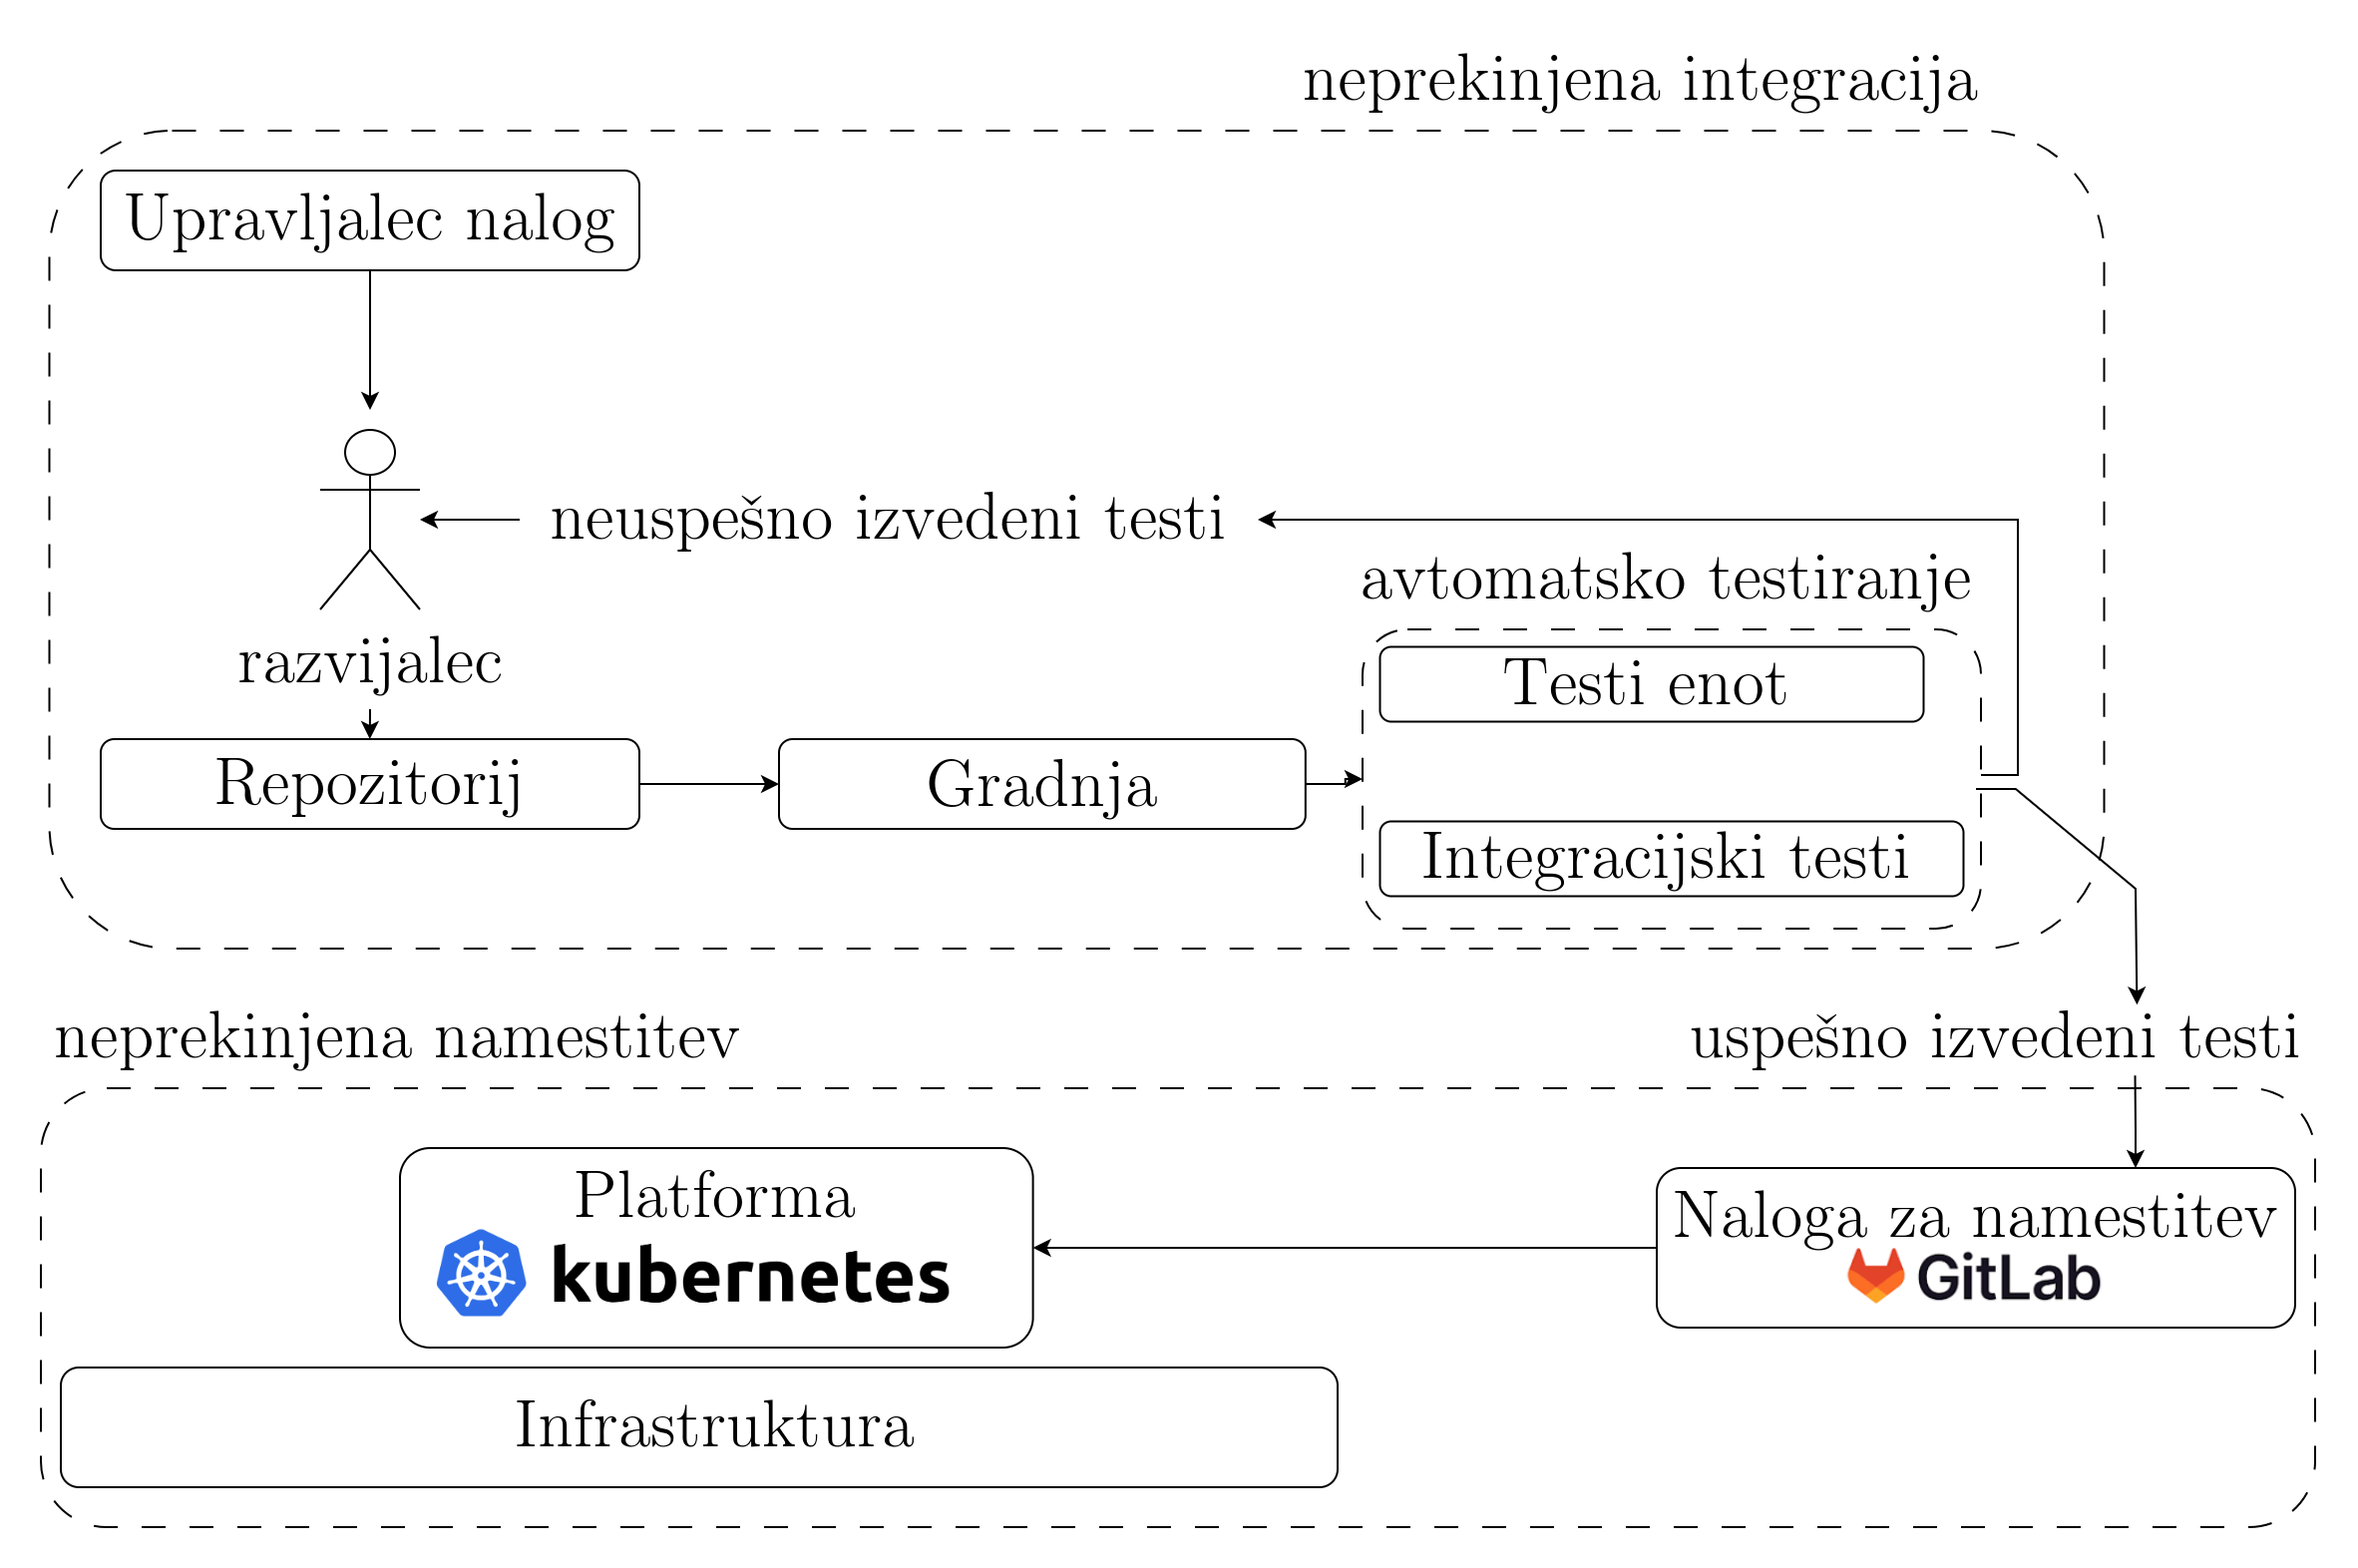
\includegraphics[scale=0.1]{figs/diagram-neprekinjene-namestitve.png}
% \caption{Pregled podatkov iz strani Kaggle.}
\label{slika1}

\end{center}
\end{figure}

\end{columns}



\note[item]{Najširši obseg pa predstavlja neprekinjena namestitev, ki je praksa razvoja
programske opreme, pri kateri se spremembe kode avtomatsko zgradijo, preizkusijo, oddajo naročniku in tudi objavijo v produkcijsko okolje brez posredovanja človeka}
\note[item]{Cilj neprekinjene namestitve je, da se nove funkcionalnosti in popravki čim hitreje dostavijo končnim uporabnikom.}
\note[item]{Da bi to dosegli, uporabljamo tehnologije za upravljanje in rezervacijo računalniških virov z uporabo datotek, ki jih računalnik zna prebrati – temu rečemo tudi infrastruktura kot koda.}
\note[item]{Eno izmed takšnih tehnologij predstavlja platforma Kubernetes, ki smo jo sami uporabili in nam omogoča, da v formatu YAML definiramo konfiguracijo namestitve naše aplikacije in jo s preprostim ukazom tudi namestimo.}

\end{frame}

%------------------------------------------------

\begin{frame}
\frametitle{GitLab}

\begin{columns}

\column{.7\textwidth} % Left column and width

\begin{itemize}
    \item porazdeljen sistem za nadzor različic
    \item velik nabor orodji za upravljanje in dostavo aplikacij
    \begin{itemize}
        \item orodja za vodenje projekta
        \item orodje za gradnjo in zagon cevovodov CI/CD
        \item orodja za pregled kode in medsebojno sodelovanje
        \item register za shranjevanje vsebniških slik
    \end{itemize}
    \item odprtokodna rešitev
    \item namestitev na lastni infrastrukturi
\end{itemize}

\column{.3\textwidth} % Right column and width
\begin{figure}[htbp]
\begin{center}

\includegraphics[scale=0.1]{figs/gitlab-logo-100.png}
\label{slika1}
% https://about.gitlab.com/press/press-kit/

\end{center}
\end{figure}

\end{columns}



\note[item]{Za izvajanje praks DevOps v našem podjetju uporabljamo platformo GitLab.}
\note[item]{Osnovni namen platforme je porazdeljen sistem za nadzor različic, ki deluje na podoben način kot orodje Git.}
\note[item]{Obenem pa nudi še veliko drugih funkcionalnosti kot so: orodja za vodenje projekta, sistem za gradnjo in zagon cevovoda neprekinjene integracije in dostave, orodja za pregled kode in medsebojno sodelovanje, register za shranjevanje vsebniških slik in podobno.}
\note[item]{Za platformo GitLab smo se v podjetju odločili predvsem ker je odprtokodna in omogoča namestitev na lastni infrastrukturi.}
\end{frame}

%------------------------------------------------

\begin{frame}
\frametitle{GitLab CI/CD}

\begin{columns}

\column{.7\textwidth} % Left column and width

\begin{itemize}
    \item orodje za gradnjo in zagon cevovodov CI/CD
    \item cevovodi, sestavljeni iz zaporedji nalog
    \item konfiguracijska datoteka \texttt{.gitlab-ci.yml}
    \item izvajalci nalog GitLab
    \item paralelno izvajanje nalog
\end{itemize}

\column{.3\textwidth} % Right column and width
\begin{center}

\begin{figure}[htbp]

\includegraphics[scale=0.15]{figs/gitlab-ci-cd-logo.png}
% https://addissoftware.com/wp-content/uploads/2020/09/gitlab-ci-cd-logo_2x-1.png
\label{slika1}
\end{figure}

\end{center}


\end{columns}

\begin{columns}
\column{.5\textwidth}
\begin{figure}[]
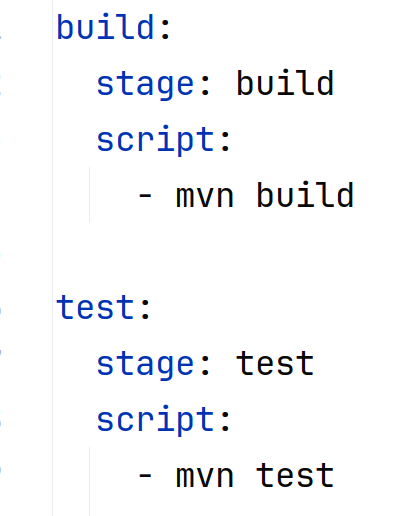
\includegraphics[scale=0.18, right]{figs/osnoven-primer-cevovoda-yaml.png}
\label{slika1}
\end{figure}
\column{.5\textwidth}
\begin{figure}[]

\includegraphics[scale=0.5, right]{figs/osnoven-primer-cevovoda.png}
\label{slika1}
\end{figure}
\end{columns}



\note[item]{Za vzpostavitev procesa neprekinjene integracije in dostave smo uporabili orodje GitLab CI/CD, ki je integrirano v platformo GitLab.}
\note[item]{Orodje temelji na konceptu cevovodov, ki so sestavljeni iz zaporedja nalog. Vsak cevovod ima lahko več faz, v katerih je nalog več nalog, vsaka naloga pa ima lahko več akcij.}
\note[item]{Cevovod definiramo v datoteki \texttt{.gitlab-ci.yml} v formatu YAML. Orodje to datoteko avtomatsko prepozna in ob vsakem odrivu kode v repozitorij kreira cevovod.}
\note[item]{Za izvajanje nalog skrbijo izvajalci nalog GitLab. Izvajajo se lahko na lastni infrastrukturi ali pa na oblačnih virtualnih strojih in omogočajo paralelno izvajanje nalog, kar lahko pohitri izvajalni čas cevovoda.}
\end{frame}

%------------------------------------------------

\begin{frame}
\frametitle{Osnoven cevovod}


\begin{figure}[htbp]
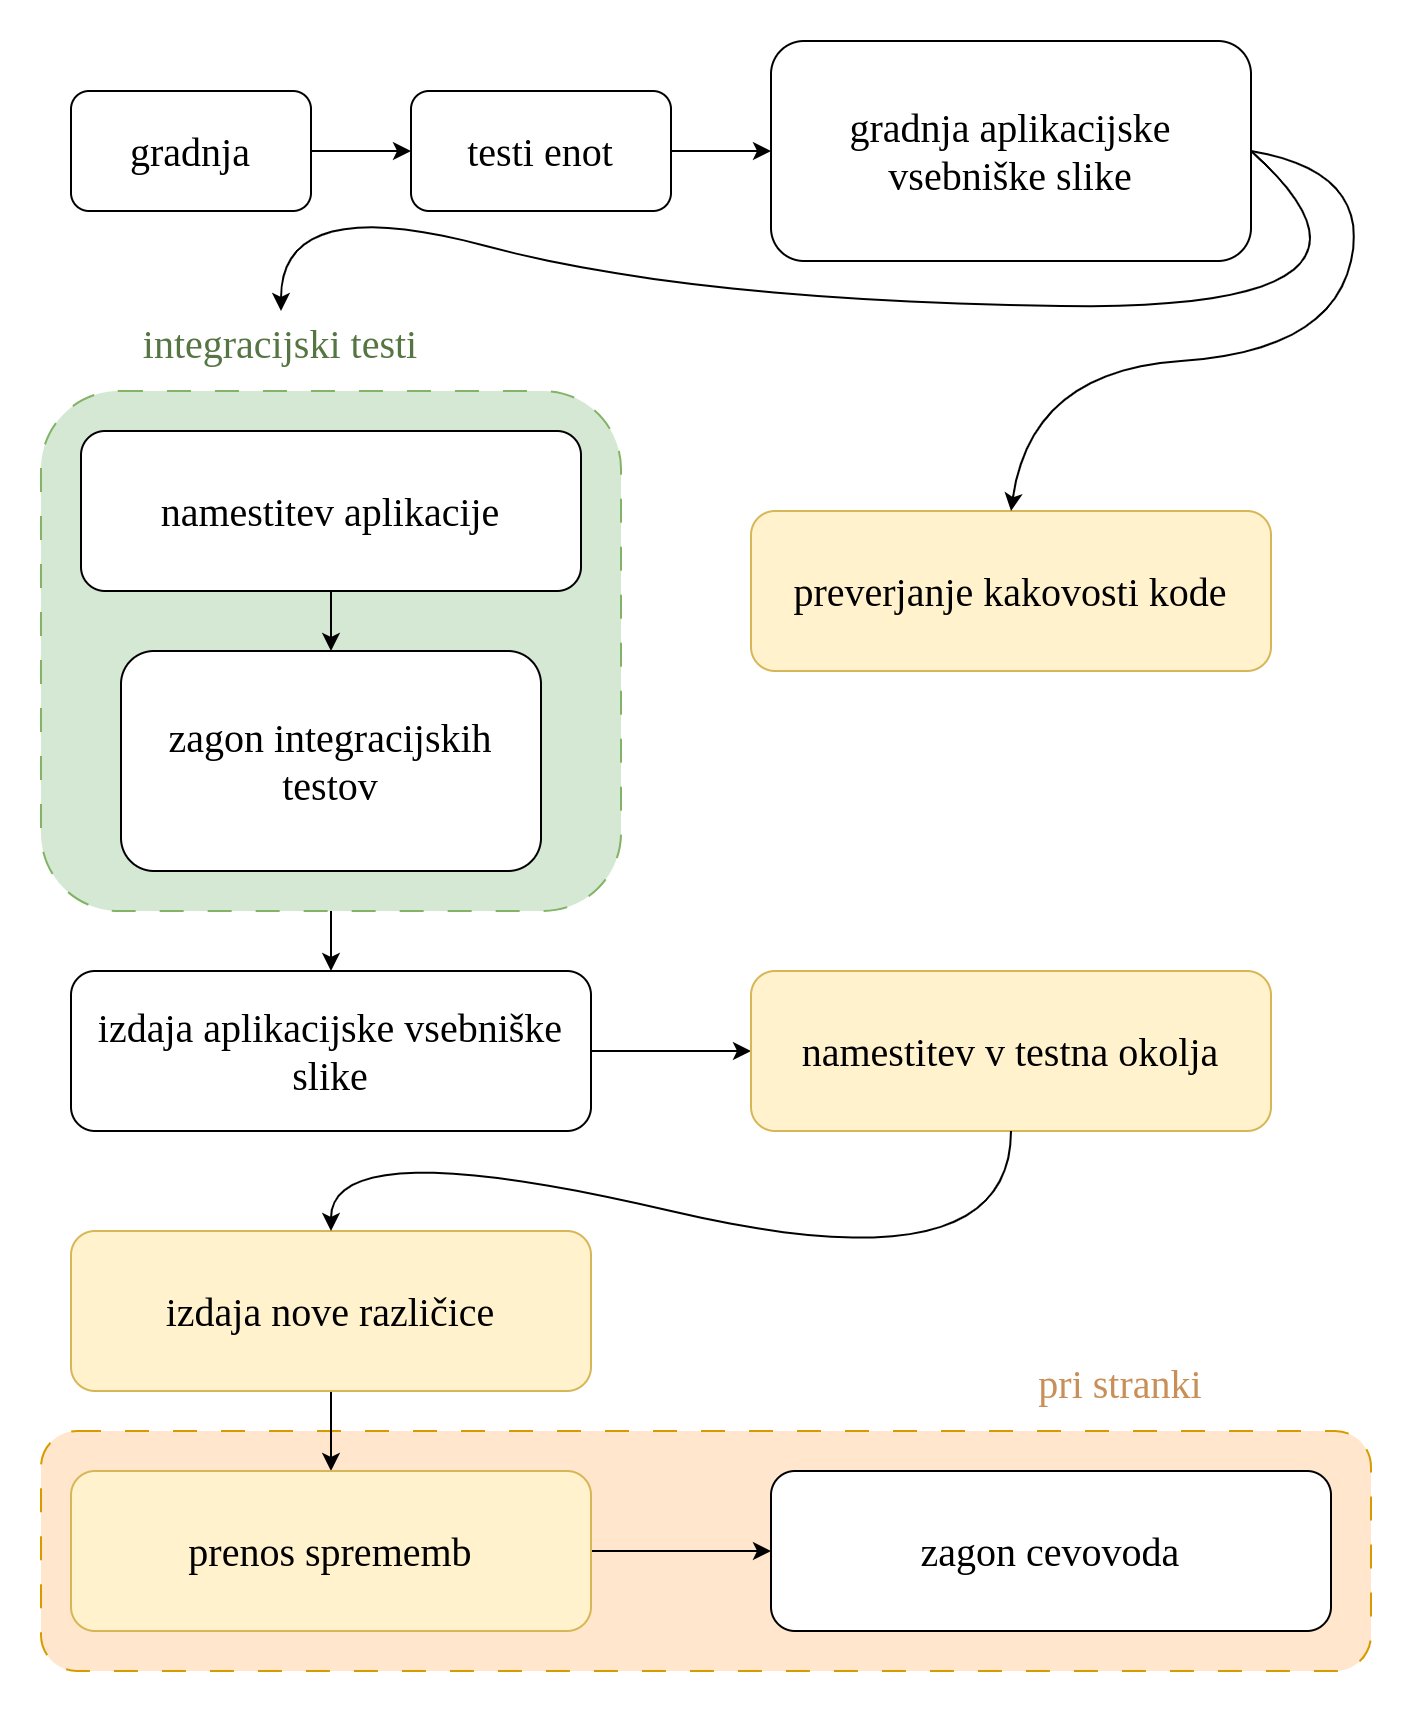
\includegraphics[scale=0.124]{figs/osnoven-cevovod.png}
\label{slika1}
\end{figure}

\note[item]{Osnoven cevovod je sestavljen iz naslednjih korakov:}
\note[item]{gradnja aplikacije}
\note[item]{zagon testov enot}
\note[item]{gradnja aplikacijske vsebniške slike, ki se uporabi za namestitev aplikacije na gručo Kubernetes, ki je namenjena izvajanju integracijskih testov}
\note[item]{vzporedno z integracijskimi testi lahko zaženemo tudi orodja za statično analizo kode}
\note[item]{če so bili vsi predhodni koraki uspešni, se aplikacijska vsebniška sika označi z ustrezno številko različice in se ustvarijo naloge za namestitev v testna okolja}
\note[item]{čisto na koncu pa so na voljo tudi naloge za izdajanje novih različic, ki jih razvijalci lahko ročno zaženejo}

\end{frame}

%------------------------------------------------

\begin{frame}
\frametitle{Izdaja nove različice in oddaja naročniku}


\begin{itemize}
    \item vse spremembe stisnemo v eno spremembo (ang. \texit{squash})
    \item naročniku avtomatsko sporočimo, da smo izdali novo različico
    \item naročnik ročno zažene nalogo za prevzem
    \item kreira se cevovod z nalogami za namestitev v naročnikova okolja
\end{itemize}

\vspace{20px}
\begin{figure}[b]
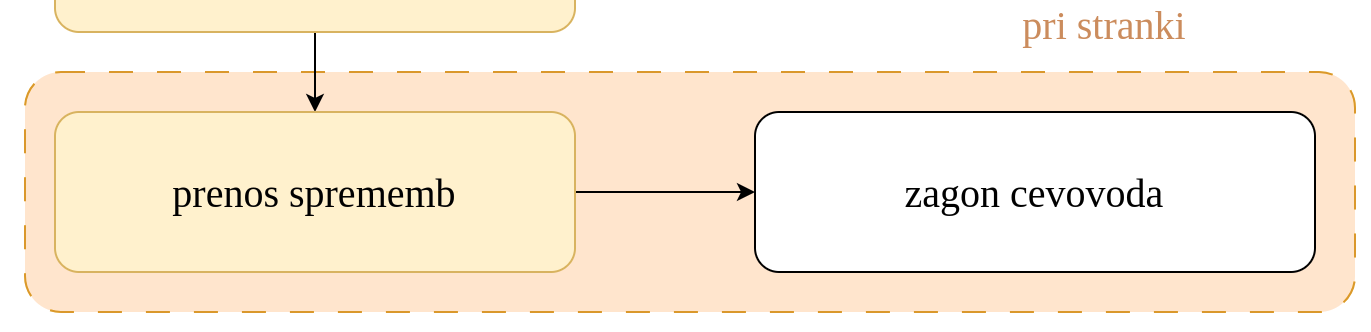
\includegraphics[scale=0.2]{figs/cevovod-pri-stranki.png}
\label{slika1}
\end{figure}

\note[item]{Da bi bil naročnik čim bolj neodvisen od podjetja, omogočimo naročniku izvajanje enakega cevovoda z manjšimi prilagoditvami.}
\note[item]{Ob izdaji nove različice vse spremembe od zadnje izdane različice stisnemo v eno spremembo in jo dodamo na posebno vejo imenovano \texttt{release} in naročniku avtomatsko sporočimo, da smo izdali novo različico.}
\note[item]{Naročniku lahko nato ročno zažene posebno nalogo, ki prenese spremembe v njegov repozitorij.}
\note[item]{Ko se sprememba uspešno presene, se zažene enak cevovod z nalogami za namestitev v naročnikova okolja.}


\end{frame}

%------------------------------------------------

\begin{frame}
\frametitle{Komponenta Medius CD}


\begin{itemize}
    \item poenotenje cevovodov, zmanjšanje količine podovojene konfiuracije in kode ter lažje vzdrževanje
    \item predloge GitLab in skripti napisani v jeziku Bash
    \item izvajalne slike - vsebniške slike za izvajanje nalog
    \item \texttt{rocky-with-tools} - osnova za gradnjo izvajalnih slik
\end{itemize}

\vspace{20px}
\begin{figure}[b]

\includegraphics[scale=0.4]{figs/medius-cd.png}
\label{slika1}
\end{figure}

\note[item]{Z željo po poenotenju obstoječih cevovodov na projektih, zmanjšanju količine podvojene konfiguracije in kode ter lažjemu vzdrževanju smo razvili komponento za vzpostavitev cevovodov neprekinjene integracije in dostave imenovano Medius CD.}
\note[item]{Sestavljena je iz dveh delov: predlog GitLab in skript, napisanih v jeziku Bash.}
\note[item]{Naloge v cevovodu poganjajo izvajalci nalog GitLab. V konfiguracijski datoteki cevovoda pa lahko nastavimo tudi vsebniško sliko, v kateri izvajalec nalogo zažene. Takšne slike imenujemo izvajalne slike in jih je potrebno najprej zgraditi in naložiti na register vsebniških slik.}
% \note[item]{Pred razvojem komponente smo izvajalne slike gradili in hranili v enem projektu. To nam je omogočalo, da smo lahko isto sliko večkrat uporabili. Kmalu pa smo ugotovili, da takšen način vodenja slik oteži vzdrževanje, saj smo morali veliko slik prilagajati posameznimi projektom.}
\note[item]{Izvajalne slike hranimo in gradimo v vsakem projektu posebej. Pripravili pa smo vsebniško sliko imenovano \texttt{rocky-with-tools}, ki vsebuje operacijski sistem Rocky Linux in orodja, ki jih potrebujemo za izvajanje cevovodov. To sliko lahko nato uporabimo za osnovo ostalih izvajalnih slik.}


\end{frame}

%------------------------------------------------

\begin{frame}
\frametitle{Datoteka \texttt{config\_file}}

\begin{columns}

\column{.5\textwidth} % Left column and width

\begin{itemize}
    \item mehanizem za nastavljanje spremenljivk v cevovodu
    \item \texttt{variables} - globalne spremenljivke
    \item \texttt{services} - seznam aplikacij
    \begin{itemize}
        % \item \texttt{variables} - spremenljivke za posamezno aplikacijo
        \item \texttt{environments} - namestitvena okolja aplikacije
        % \begin{itemize}
        %     \item \texttt{variables} - spremenljivke za posamezno okolje
        % \end{itemize}
    \end{itemize}
    \item \texttt{it} - konfiguracija okolja za zagon integracijskih testov
    % \begin{itemize}
    %     \item \texttt{variables} - spremenljivke za integracijske teste
    %     \item \texttt{deployments} - seznam aplikacij za integracijske teste
    % \end{itemize}
\end{itemize}


\column{.5\textwidth}
\begin{figure}[b]
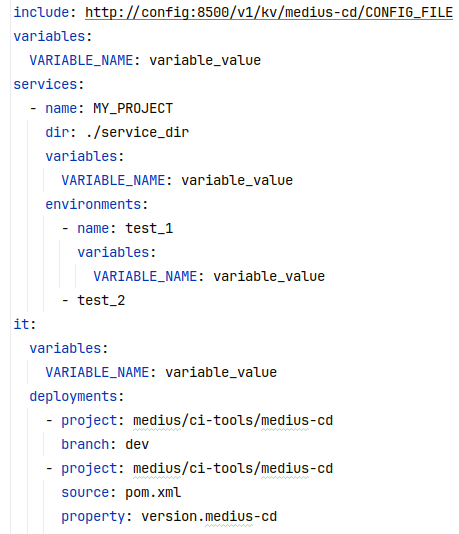
\includegraphics[scale=0.37]{figs/config_file.png}
\label{slika1}
\end{figure}

\end{columns}

\note[item]{Za prilagajanje razvitega cevovoda projektnim specifikam smo razvili mehanizem za nastavljanje spremenljivk cevovoda preko datoteke \texttt{config\_file} v formatu YAML.}
\note[item]{Datoteko na začetku cevovoda prenesemo iz konfiguracijskega strežnika Consul ali spremenljivke GitLab.}
\note[item]{Vsebuje naslednje lastnosti:}
\note[item]{\texttt{variables} - globalne spremenljivke, ki so na voljo v vseh nalogah}
\note[item]{\texttt{services} - seznam aplikacij, za katere želimo zgraditi vsebniške slike.}
\note[item]{vsaki aplikacij lahko nastavimo še spremenljivke specifične za aplikacijo in namestitvena okolja}
\note[item]{ter za vsako namestitveno okolje spremenljivke specifične za tisto okolje}
\note[item]{na koncu lahko nastavimo tudi konfiguracijo namestitve odvisnih aplikacij, potrebnih za zagon integracijskih testov.}


\end{frame}

%------------------------------------------------

\begin{frame}
\frametitle{Naloge GitLab}


\begin{columns}

\column{.5\textwidth} % Left column and width

\begin{itemize}
    \item format YAML
    \item del \texttt{script} definira lupinski skript, ki ga naloga izvede
    \item za kompleksnejše naloge uporabimo samostojne skripte v jeziku Bash
    \item več manjših predlog Gitlab
    \item dodajanje predlog s ključno besedo \texttt{include}
\end{itemize}


\column{.5\textwidth}
\begin{figure}[b]

\includegraphics[scale=0.27]{figs/hello_world_2.png}
\label{slika1}
\end{figure}

\begin{figure}[b]
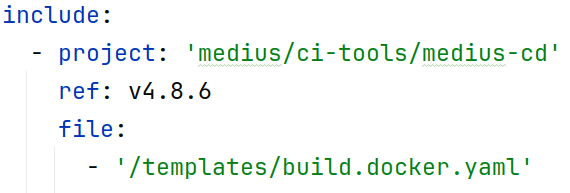
\includegraphics[scale=0.27]{figs/include.png}
\label{slika1}
\end{figure}

\end{columns}

\note[item]{Naloge GitLab definiramo v formatu YAML.}
\note[item]{Najbolj preprosta naloga je sestavljena iz imena naloge in dela \texttt{script}, ki vsebuje lupinski skript, ki ga naloga izvede.}
% \note[item]{Delovanje naloge pa lahko prilagajamo še z drugimi atributi.}
\note[item]{Logiko kompleksnejših nalog pa smo definirali v samostojnih skriptah, napisanih v jeziku Bash, ki jih lahko tudi testiramo in uporabimo na več mestih}
\note[item]{V okviru cevovoda projekta Medius CD te skripte zapakiramo v različne formate, ki jih naložimo na centralni repozitorij Nexus.}
\note[item]{Ker pa se projekti močno razlikujejo, smo pripravili več manjših predlog GitLab, ki jih lahko večkrat uporabimo, da ustvarimo različne cevovode.}
\note[item]{Pripravljene predloge se nahajajo v repozitoriju projekta Medius CD in jih lahko v ostale projekte dodamo s ključno besedo \texttt{include}.}



\end{frame}

%------------------------------------------------

\begin{frame}
\frametitle{Vtičnik GitLab Template Lint}

\begin{itemize}
    \item uporaba predlog oteži razhroščevanje
    \item vtičnik za integrirano okolje IntelliJ IDEA
    \item klic na GitLab API za preverjanje pravilnosti predloge
    \item prikaz združene konfiguracije
\end{itemize}


\begin{figure}[b]
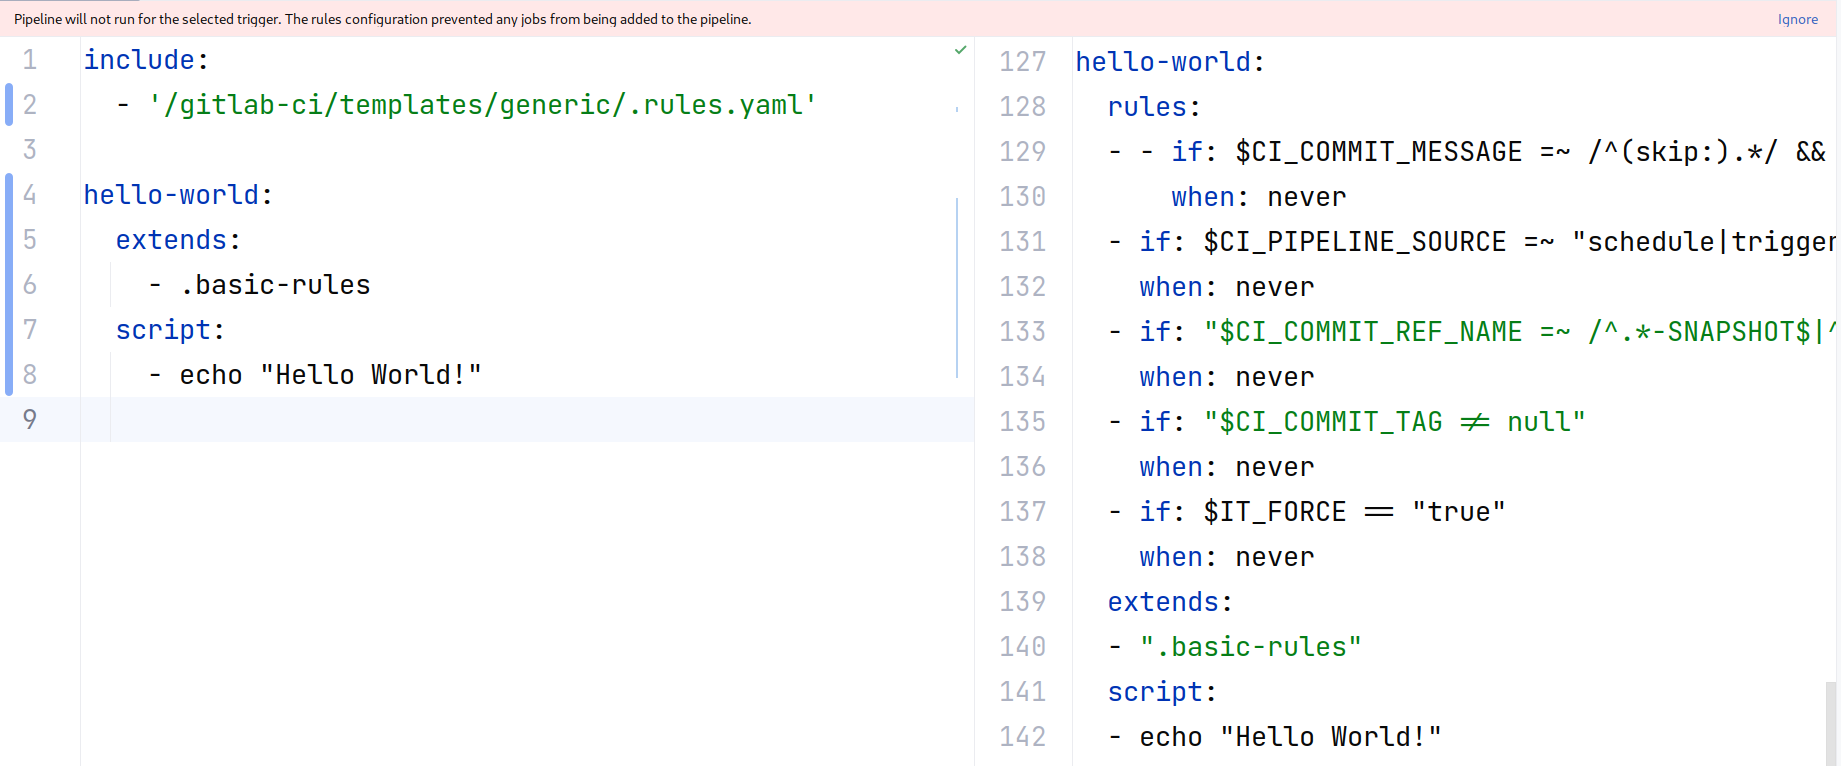
\includegraphics[scale=0.18]{figs/gitlab-template-lint-primer-1.png}
\label{slika1}
\end{figure}


\note[item]{Z uporabo predlog pa smo otežili razhroščevanje predlog.}
\note[item]{Zato smo se odločili, da razvijemo vtičnik za integrirano okolje Intellij IDEA, s katerim dodamo funkcionalnost za preverjanje pravilnosti konfiguracijskih datotek GitLab.}
\note[item]{Vtičnik zgolj pošlje vsebino trenutno odprte predloge GitLab programskemu vmesniku platforme GitLab, ki preveri pravilnosti datoteke in v odgovoru vrne morebitne napake ter vsebino združene konfiguracijske datoteke.}
\note[item]{Vtičnik napake prikaže na vrhu urejevalnika združeno vsebino pa na desni strani urejevalnika.}


\end{frame}

%------------------------------------------------

\begin{frame}
\frametitle{Cevovod aplikacije}


\begin{columns}

\column{.5\textwidth} % Left column and width

\begin{itemize}
    \item imenik \texttt{runner-images}
    \item imenik \texttt{deploy/docker}
    \item imenik \texttt{deploy/k8s}
    \item datoteka \texttt{.gitlab-ci.yml}
    \item imenik \texttt{.gitlab}, ki vsebuje datoteki \texttt{.build-runners.yml} in \texttt{.main.yml}
\end{itemize}

\column{.5\textwidth}
\begin{figure}[b]
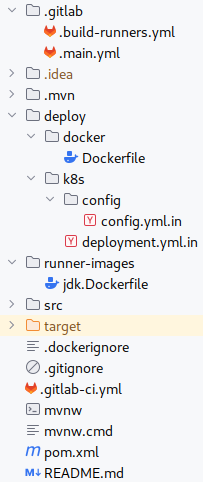
\includegraphics[scale=0.4]{figs/direktorijska_struktura.png}
\label{slika1}
\end{figure}

\end{columns}

\note[item]{Z novo razvito komponento je cevovod enostavno dodati. V korenski imenik dodamo:}
\note[item]{imenik \texttt{runner-images}, z datotekami, ki definirajo izvajalne slike.}
\note[item]{imenik \texttt{deploy/docker}, z datoteko, ki definira aplikacijsko vsebniško sliko}
\note[item]{imenik \texttt{deploy/k8s}, s predlogami, ki vsebujejo konfiguracijo za namestitev na gručo na platformi Kubernetes}
\note[item]{vnaprej pripravljeno datoteko \texttt{.gitlab-ci.yml}, ki je za vse projekte enaka}
\note[item]{imenik \texttt{.gitlab}, z datotekama \texttt{.build-runners.yml}, ki uporabi predlogo za gradnjo izvajalnih slik in \texttt{.main.yml}, ki uporabi predlogo aplikacijskega cevovoda}

\end{frame}

%------------------------------------------------

\begin{frame}
\frametitle{Študija primera: projekt v programskem jeziku Java}


% \begin{columns}

% \column{.5\textwidth} % Left column and width

\begin{itemize}
    \item pridobivanje podatkov o izvedenih denarnih transakcijah podjetja
    \item uporabljene tehnologije:
    \begin{itemize}
        \item programski jezik Java
        \item orodje Maven
        \item aplikacijski strežnik Wildfly
        \item podatkovna baza Oracle
    \end{itemize}
    \item izvajalec nalog zaradi varnosti nima dostopa do interneta
\end{itemize}

% \column{.5\textwidth}
% \begin{figure}[b]
% 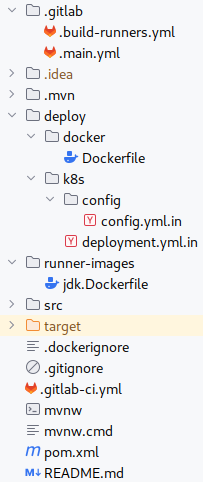
\includegraphics[scale=0.4]{figs/direktorijska_struktura.png}
% \label{slika1}
% \end{figure}

% \end{columns}

\note[item]{Sedaj bom predstavil delovanje cevovoda na resničnem projektu, ki omogoča pridobivanje podatkov o izvedenih denarnih transakcijah nekega podjetja.}
\note[item]{Aplikacija je napisana v programskem jeziku Java, za gradnjo uporablja orodje Maven, za delovanje uporablja aplikacijski strežnik Wildfly in za shranjevanje podatkov podatkovno bazo Oracle.}
\note[item]{Naročnik projekta, je zaradi varnosti zahteval, da se celoten cevovod izvaja brez povezave na internet.}
\note[item]{To pomeni, da morajo biti vse odvisnosti projekta dostopne preko internih repozitorijev in registrov, do katerih skripti v nalogah lahko dostopajo.}

\end{frame}

%------------------------------------------------

\begin{frame}
\frametitle{Študija primera: \texttt{config\_file}}


% \begin{columns}

% \column{.5\textwidth} % Left column and width

\begin{figure}[b]
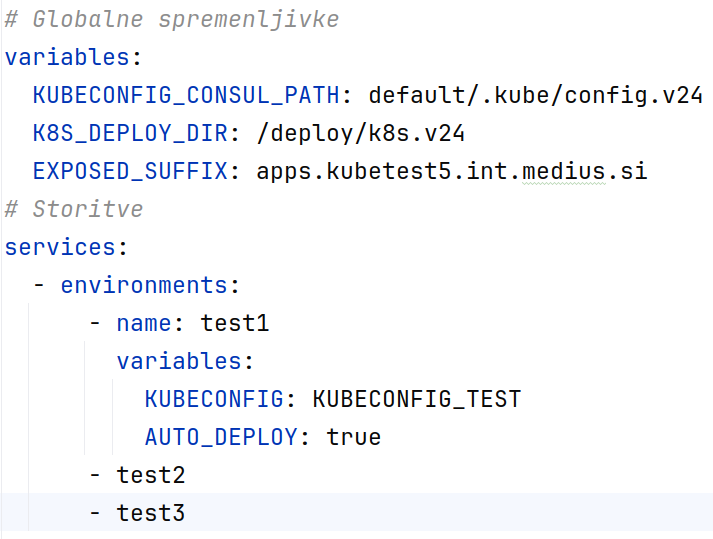
\includegraphics[scale=0.4]{figs/java_config.png}
\label{slika1}
\end{figure}

% \column{.5\textwidth}
% \begin{figure}[b]
% 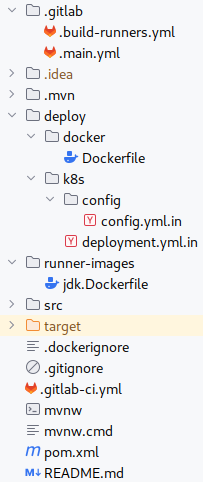
\includegraphics[scale=0.4]{figs/direktorijska_struktura.png}
% \label{slika1}
% \end{figure}

% \end{columns}

\note[item]{Najprej smo pripravili konfiguracijsko datoteko \texttt{config\_file}, ki izgleda nekako takole:}
\note[item]{Nastavili smo pot do konfiguracijske datoteke, ki vsebuje podatke za povezavo in avtentikacijo na platformo Kubernetes.}
\note[item]{Spremenili smo pot do imenika v repozitoriju, kjer se nahajajo konfiguracijske datoteke za namestitev na gručo platforme Kubernetes.}
\note[item]{Nastavili smo pripono spletnega naslova, na kateri bo aplikacija dostopna.}
\note[item]{Na koncu pa smo definirali različna testna okolja, v katera želimo aplikacijo namestiti.}
\note[item]{Pri naročniku se uporablja enak cevovod, vendar brez uporabe konfiguracijskega strežnika Consul, zato morajo vse datoteke, ki se sicer privzeto prenesejo s konfiguracijske strežnika, shraniti v spremenljivke GitLab.}
\end{frame}

%------------------------------------------------

\begin{frame}
\frametitle{Študija primera: izvajalne slike}


% \begin{columns}

% \column{.5\textwidth} % Left column and width

\begin{itemize}
    \item ročno prenesemo \texttt{kaniko-tools} in \texttt{rocky-with-tools}
    \item nastavimo \texttt{DOCKER\_BUILDER\_IMAGE} in \texttt{DOCKER\_FROM\_REGISTRY}
    \item dodamo datoteki:
    \begin{itemize}
        \item \texttt{jdk} - Java in Maven
        \item \texttt{wildfly} - aplikacijski strežnik Wildfly
    \end{itemize}
    \item pod ključno besedo \texttt{FROM} uporabimo spremenljivko \texttt{DOCKER\_FROM\_REGISTRY}
\end{itemize}

\vspace{20px}
\begin{figure}[b]
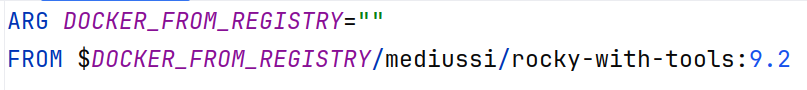
\includegraphics[scale=0.4]{figs/from_registry.png}
\label{slika1}
\end{figure}

% \column{.5\textwidth}
% \begin{figure}[b]
% 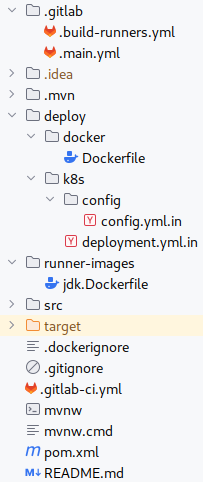
\includegraphics[scale=0.4]{figs/direktorijska_struktura.png}
% \label{slika1}
% \end{figure}

% \end{columns}

\note[item]{Ker izvajalec nalog GitLab nima dostopa do interneta, smo najprej ročno prenesli vsebniški sliki \texttt{kaniko-tools} in \texttt{rocky-with-tools} in ju naložili v register slik, ki je dostopen v izvajalcu nalog.}
\note[item]{Nastavili smo tudi spremenljivki GitLab \texttt{DOCKER\_BUILDER\_IMAGE} in \texttt{DOCKER\_FROM\_REGISTRY}, ki izvajalcu nalog povesta kje se naloženi sliki nahajata.}
\note[item]{Nato dodamo datoteki, ki definirata dve izvajalni sliki:}
\note[item]{\texttt{jdk}, ki vsebuje razvojno okolje Java in orodje Maven in se uporablja za zagon vseh nalog v cevovodu}
\note[item]{in \texttt{wildfly}, ki se uporablja za osnovo gradnje aplikacijske vsebniške slike in vsebuje aplikacijski strežnik Wildfly.}
\note[item]{V obeh datoteka pa pod ključno besedo \texttt{FROM} za predpono osnovne slike nastavimo \texttt{DOCKER\_FROM\_REGISTRY}, ki se pri gradnji slik poda kot argument.}
\note[item]{Na ta način se pri gradnji vsebniških slik za osnovo uporabijo slike iz registra, ki je dostopen v izvajalcu nalog GitLab.}
\end{frame}

%------------------------------------------------

\begin{frame}
\frametitle{Študija primera: konfiguracijske datoteke cevovoda}


% \begin{columns}

% \column{.5\textwidth} % Left column and width

\begin{figure}[b]
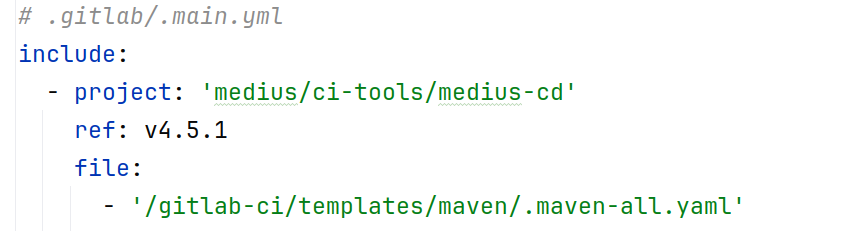
\includegraphics[scale=0.3]{figs/template_1.png}
\label{slika1}
\end{figure}

\begin{figure}[b]
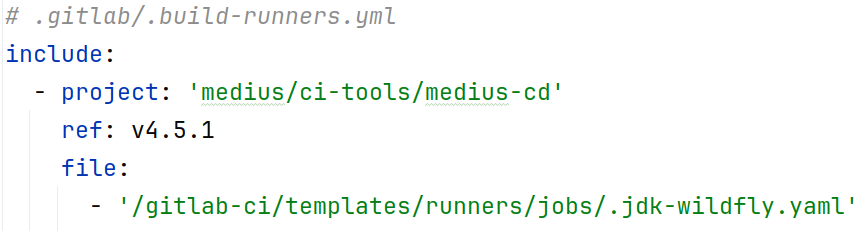
\includegraphics[scale=0.3]{figs/tempalte_2.png}
\label{slika1}
\end{figure}

% \column{.5\textwidth}
% \begin{figure}[b]
% 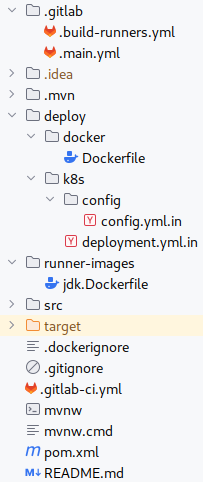
\includegraphics[scale=0.4]{figs/direktorijska_struktura.png}
% \label{slika1}
% \end{figure}

% \end{columns}

\note[item]{Za definicijo cevovoda smo v korenski imenik dodali datoteko \texttt{.gitlab-ci.yml} in uporabili predlogi komponente Medius CD, ki smo ju dodali v datoteki v imeniku \texttt{.gitlab}.}
\note[item]{V datoteki \texttt{.main.yml} smo uporabili predlogo za cevovod projekta, ki uporablja programski jezik Java in orodje Maven.}
\note[item]{V datoteki \texttt{.build-runners.yml} pa smo uporabili predlogo za cevovod gradnje izvajalnih slik \texttt{jdk} in \texttt{wildfly}.}
\note[item]{Cevovod gradnje izvajalnih slik zaženemo tako, da pred zagonom cevovoda nastavimo spremenljivko \texttt{BUILD\_RUNNERS} na \texttt{true}}.
\note[item]{Nato lahko zaženemo cevovod aplikacije, ki je sestavljen iz naslednjih nalog:}
\end{frame}

%------------------------------------------------

\begin{frame}
\frametitle{Študija primera: cevovod aplikacije}


% \begin{columns}

% \column{.5\textwidth} % Left column and width

\begin{figure}[b]
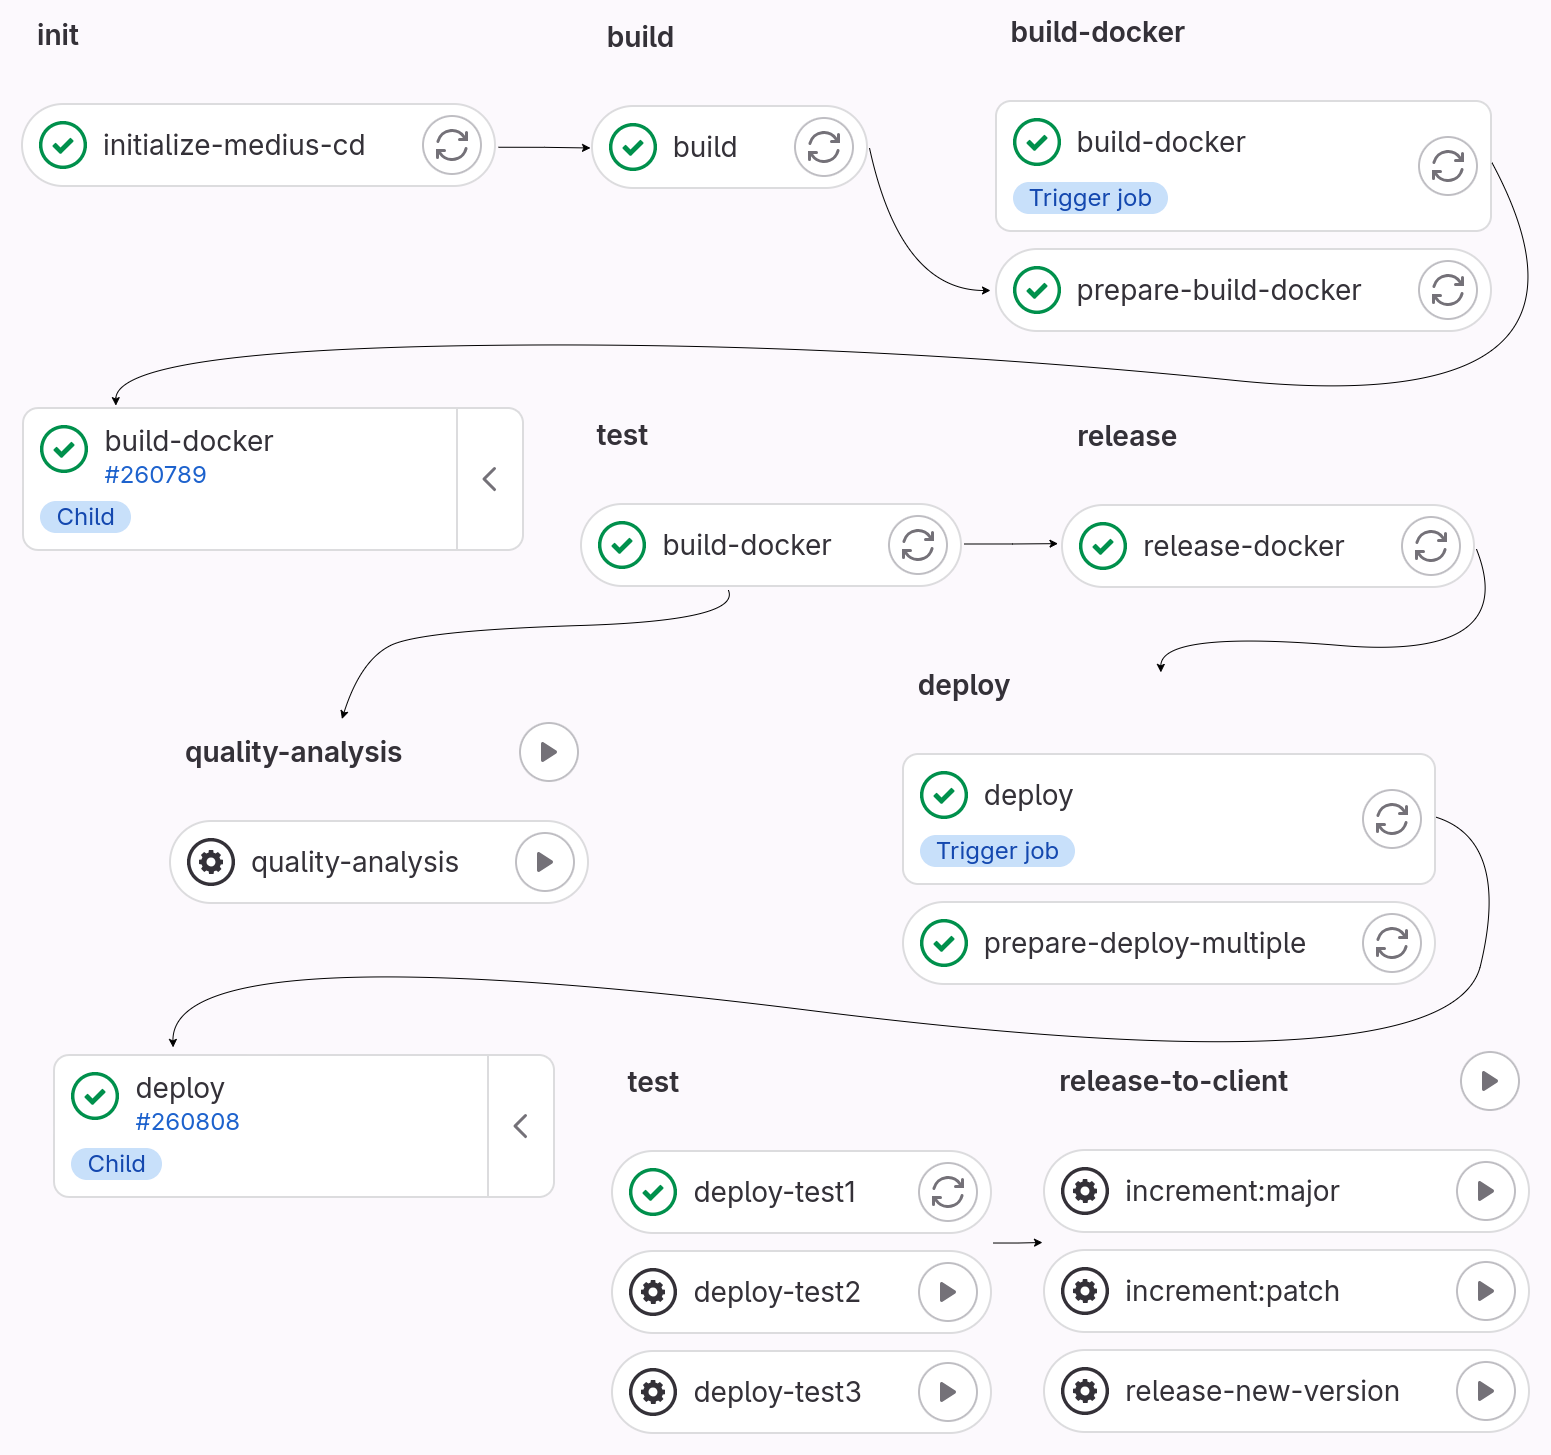
\includegraphics[scale=0.15]{figs/java-cevovod.png}
\label{slika1}
\end{figure}

% \column{.5\textwidth}
% \begin{figure}[b]
% 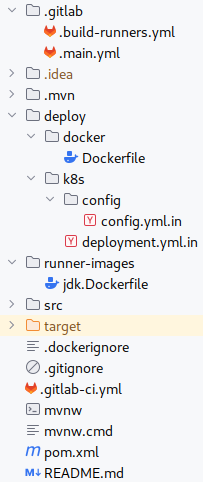
\includegraphics[scale=0.4]{figs/direktorijska_struktura.png}
% \label{slika1}
% \end{figure}

% \end{columns}

\note[item]{Priprava komponente Medius CD, ki prenese paket komponente s centralnega repozitorija Nexus in nastavi spremenljivke, ki so nastavljene v konfiguracijski datoteki \texttt{config\_file}.}
\note[item]{Gradnja aplikacije z orodjem Maven.}
\note[item]{Gradnja aplikacijske slike.}
\note[item]{Na tem mestu je tudi možno zagnati nalogo za preverjanje kakovosti kode.}
\note[item]{Izdaja nove različice aplikacijske slike.}
\note[item]{Naloga, ki kreira nove naloge za namestitev v testna okolja.}
\note[item]{In na koncu še naloge za izdajo nove različice aplikacije.}

\end{frame}

%------------------------------------------------

\begin{frame}
\frametitle{Rezultati}


% \begin{columns}

% \column{.5\textwidth} % Left column and width

\begin{itemize}
    \item opisali poslovno kritične aplikacije in proces CI/CD
    \item razvili komponento Medius CD
    \item uvedli konfiguracijsko datoteko \texttt{config\_file}
    \item omogočili podpora za različne programske jezike
    \item predstavili uporabo komponente na resničnih projektih
    \item razvili vtičnik GitLab Template Lint za integrirano razvojno okolje IntelliJ
\end{itemize}

% \column{.5\textwidth}
% \begin{figure}[b]
% 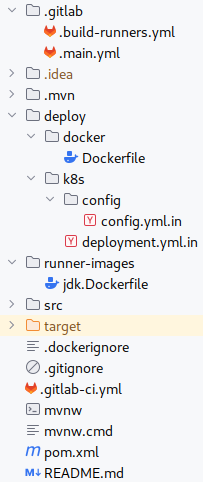
\includegraphics[scale=0.4]{figs/direktorijska_struktura.png}
% \label{slika1}
% \end{figure}

% \end{columns}

\note[item]{V okviru magistrske naloge smo opisali poslovno kritične aplikacije, predstavili proces neprekinjene integracije in dostave ter pojasnili zakaj predstavlja pomemben del pri razvoju poslovno kritičnih aplikacij.}
\note[item]{Na platformi GitLab smo razvili komponento za vzpostavitev neprekinjene integracije in dostave, imenovano Medius CD, s katero smo poenotili cevovode, zmanjšali količino podvojene konfiguracije in kode ter olajšali vzdrževanje.}
\note[item]{Uvedli smo konfiguracijsko datoteko \texttt{config\_file}, s katero smo olajšali vzdrževanje spremenljivk in dosegli visoko nivojsko abstrakcijo neprekinjene integracije in dostave tako v razvojnem okolju in okolju naročnika.}
\note[item]{Z razvito komponento smo podprli tri programske jezike.}
\note[item]{Uporabo komponente smo predstavili na cevovodih treh resničnih projektov in na ta način pokazali njeno praktično uporabnost.}
\note[item]{Razvili smo vtičnik Gitlab Template Lint za integrirano razvojno okolje IntelliJ, ki ga uporablja širša skupina razvijalcev DevOps po vsem svetu.}

\end{frame}

%------------------------------------------------

\begin{frame}
\frametitle{Zaključek}


% \begin{columns}

% \column{.5\textwidth} % Left column and width

\begin{itemize}
    \item orodje \texttt{kustomize}
    \item podpora za \texttt{Podman}, \texttt{Buildah}, \texttt{BuildKit}, \texttt{containerd}
    \item vodenje različic izvajalnih slik
\end{itemize}

% \column{.5\textwidth}
% \begin{figure}[b]
% 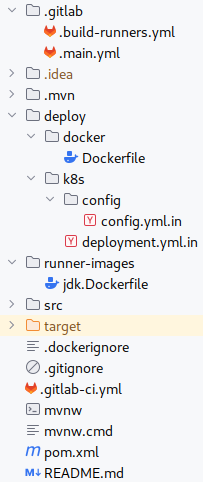
\includegraphics[scale=0.4]{figs/direktorijska_struktura.png}
% \label{slika1}
% \end{figure}

% \end{columns}

\note[item]{Razvita komponenta je zelo stabilna in že v uporabi, kljub temu pa ima še veliko prostora za izboljšave.}
\note[item]{Skript, ki ga uporabljamo za ustvarjanje konfiguracijskih datotek za namestitev na gručo Kubernetes bi lahko nadomestili z orodjem \texttt{kustomize}}
\note[item]{Trenutno so cevovodi pripravljeni za gradnjo vsebnikov z orodjema kaniko in Docker, lahko pa bi podprli tudi druga orodja, kot so Podman, Buildah, BuildKit, containerd.}
\note[item]{Pomemben manjkajoči del pa predstavlja tudi vodenje različic izvajalnih slik. Trenutno izvajalne slike redno posodabljamo brez spreminjanja številke različice. To lahko privede do težav, če želimo zagnati cevovod aplikacije, ki je starejše različice.}

\end{frame}


%------------------------------------------------

\begin{frame}{}
  \centering \Large
  \emph{Hvala za Vašo pozornost.}
\end{frame}

%\begin{frame}
%\frametitle{Multiple Columns}
%\begin{columns}[c] % The "c" option specifies %centered vertical alignment while the "t" %option is used for top vertical alignment

%\column{.45\textwidth} % Left column and width
%\textbf{Heading}
%\begin{enumerate}
%\item Statement
%\item Explanation
%\item Example
%\end{enumerate}

%\column{.5\textwidth} % Right column and width
%Lorem ipsum dolor sit amet, consectetur adipiscing elit. Integer lectus nisl, ultricies in feugiat rutrum, porttitor sit amet augue. Aliquam ut tortor mauris. Sed volutpat ante purus, quis accumsan dolor.

%\end{columns}
%\end{frame}

%------------------------------------------------

%\begin{frame}
%\frametitle{Table}
%\begin{table}
%\begin{tabular}{l l l}
%\toprule
%\textbf{Treatments} & \textbf{Response 1} & %\textbf{Response 2}\\
%\midrule
%Treatment 1 & 0.0003262 & 0.562 \\
%Treatment 2 & 0.0015681 & 0.910 \\
%Treatment 3 & 0.0009271 & 0.296 \\
%\bottomrule
%\end{tabular}
%\caption{Table caption}
%\end{table}
%\end{frame}

%------------------------------------------------

%\begin{frame}
%\frametitle{Theorem}
%\begin{theorem}[Mass--energy equivalence]
%$E = mc^2$
%\end{theorem}
%\end{frame}

%------------------------------------------------

%\begin{frame}[fragile] % Need to use the fragile option when verbatim is used in the slide
%\frametitle{Verbatim}
%\begin{example}[Theorem Slide Code]
%\begin{verbatim}
%\begin{frame}
%\frametitle{Theorem}
%\begin{theorem}[Mass--energy equivalence]
%$E = mc^2$
%\end{theorem}
%\end{frame}\end{verbatim}
%\end{example}
%\end{frame}

%------------------------------------------------

%\begin{frame}
%\frametitle{Figure}
%Uncomment the code on this slide to include your own image from the same directory as the template .TeX file.
%\begin{figure}
%\includegraphics[width=0.8\linewidth]{test}
%\end{figure}
%\end{frame}

%------------------------------------------------

%\begin{frame}[fragile] % Need to use the fragile option when verbatim is used in the slide
%\frametitle{Citation}
%An example of the \verb|\cite| command to cite within the presentation:\\~

%This statement requires citation \cite{p1}.
%\end{frame}

%------------------------------------------------

%\begin{frame}
%\frametitle{References}
%\footnotesize{
%\begin{thebibliography}{99} % Beamer does not support BibTeX so references must be inserted manually as below
%\bibitem[Smith, 2012]{p1} John Smith (2012)
%\newblock Title of the publication
%\newblock \emph{Journal Name} 12(3), 45 -- 678.
%\end{thebibliography}
%}
%\end{frame}

%------------------------------------------------

% \begin{frame}
% \Huge{\centerline{Hvala za pozornost.}}
% \end{frame}

%----------------------------------------------------------------------------------------

\end{document} 